% 图 11.1 —— 由 `checks/emit_hand.py` 自动拼出（probe 精测 + prims2 图元分解）
%%
% ⚠ 这是**稿子不是成品**：跑 `checks/checkhand.py 11.1` 看指标 + 看叠合图。
%%
%% ⚠ 待核：
%   · 本图 probe 报出阴影族 1 个 —— **本脚本不生成阴影**（要照原书手写）；prims2 的 strokes 里可能含阴影线，核对时留意别画重
%   · 可疑字形 2 项（空心圈 ⊙ 常被认成字母 o）—— 见文件末
%%
\documentclass[12pt]{standalone}
\usepackage{fontspec}
\setsansfont{Arial}
\newfontfamily\mfallback{DejaVu Sans}
\usepackage{tikz}
\begin{document}
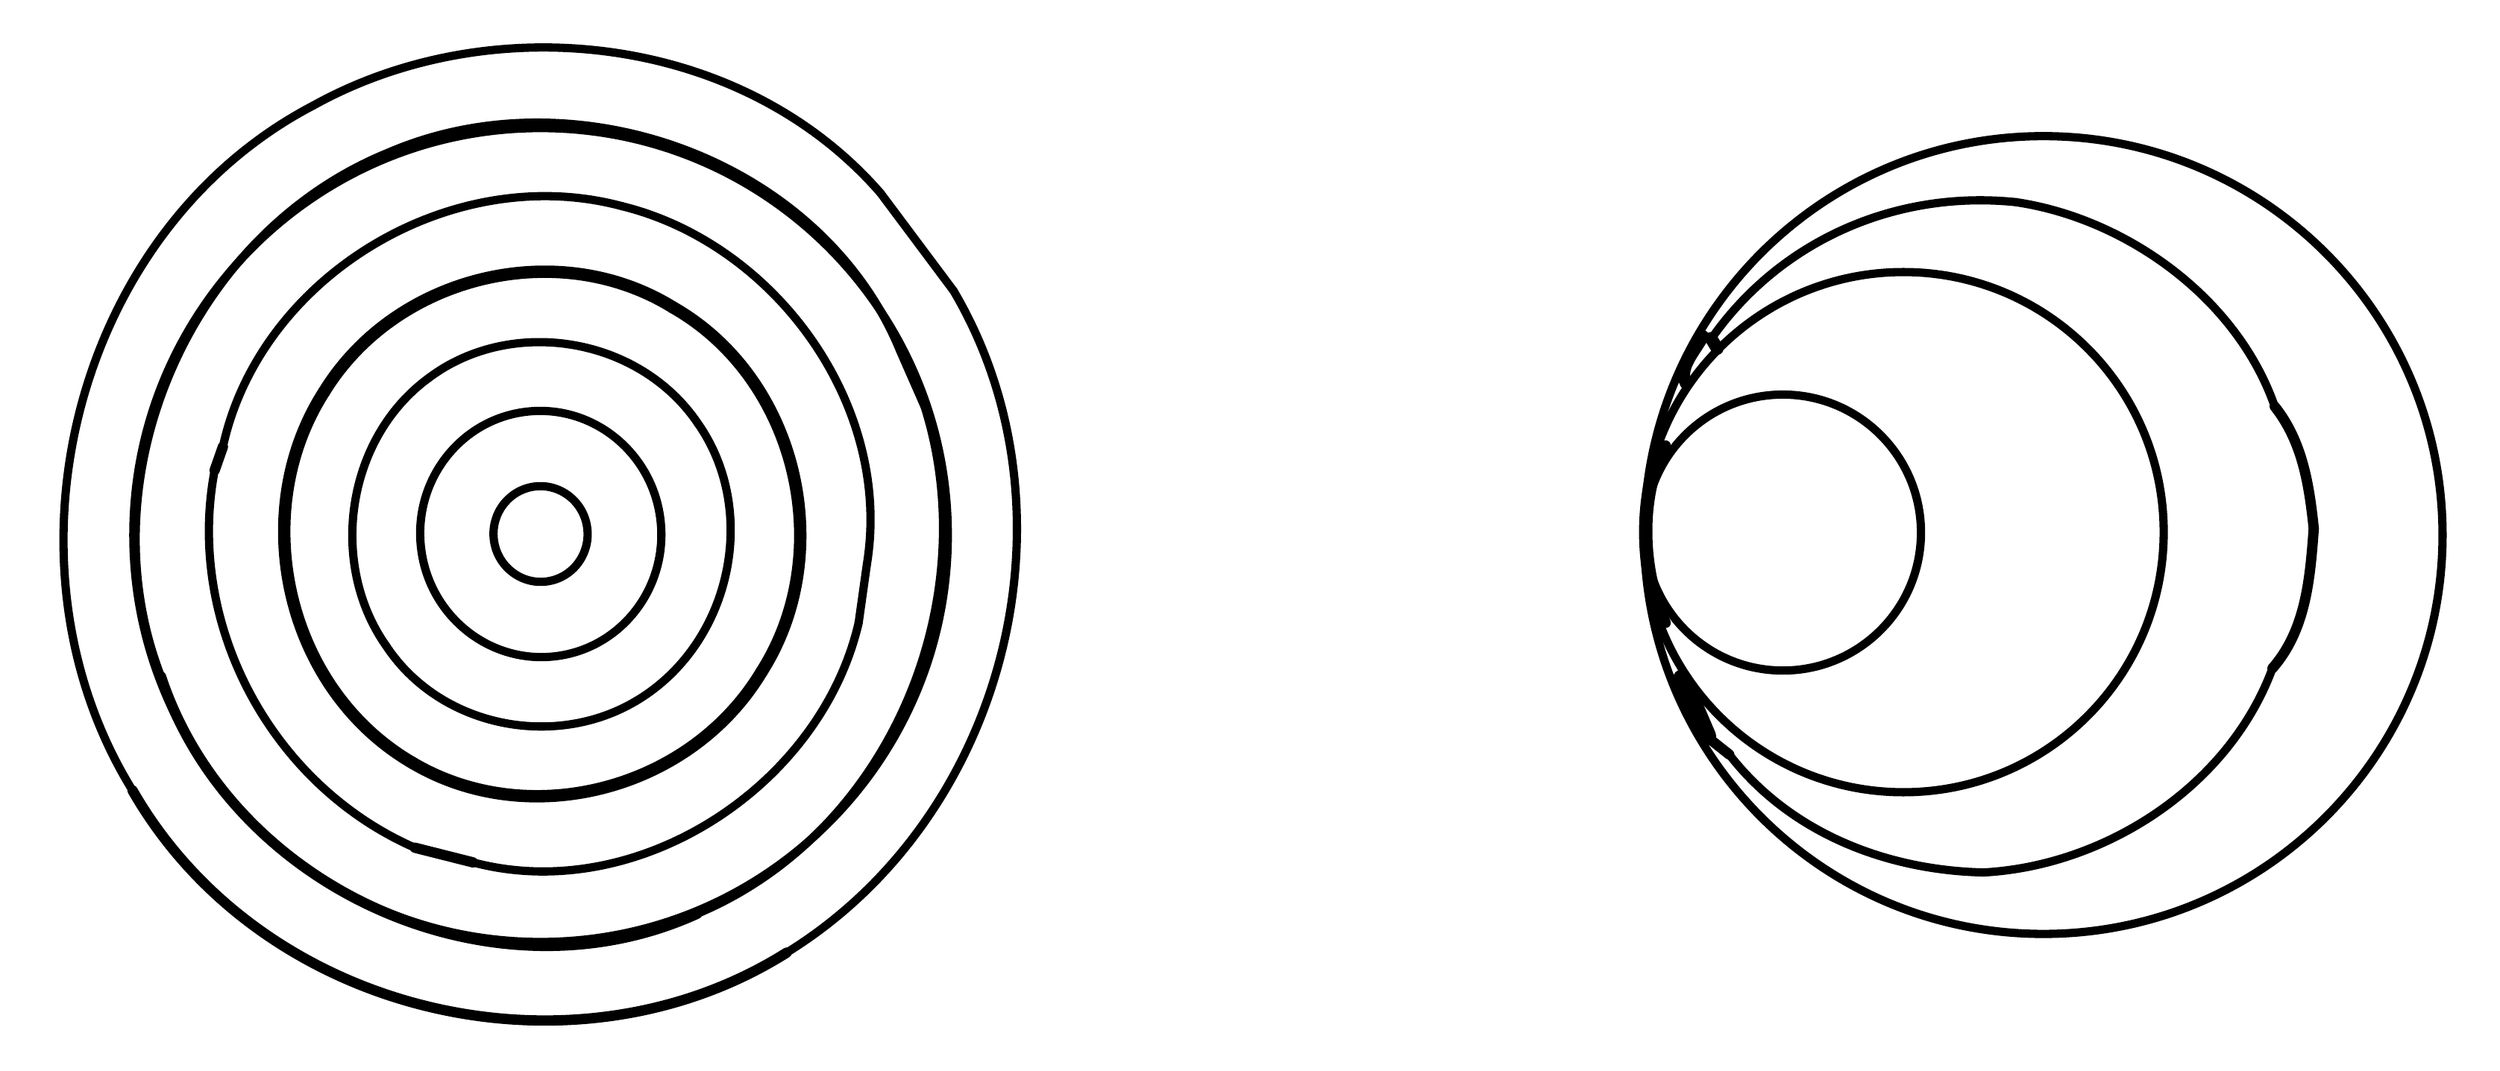
\begin{tikzpicture}[x=1pt, y=-1pt, line width=4.0pt, line cap=round, line join=round]

  %% ════ 直线段（prims2 的 strokes）════
  \draw[line width=6.1pt] (822.0,159.0) -- (819.0,154.0);
  \draw[line width=9.0pt] (817.0,347.0) -- (805.0,319.0);
  \draw[line width=5.0pt] (818.0,348.0) -- (827.8,355.8);
  \draw[line width=4.0pt] (426.1,160.1) -- (438.0,187.2);
  \draw[line width=4.0pt] (452.0,131.0) -- (416.6,83.6);
  \draw[line width=4.0pt] (406.0,292.0) -- (410.0,263.6);
  \draw[line width=5.0pt] (98.0,206.6) -- (94.0,218.0);
  \draw[line width=5.0pt] (191.0,401.0) -- (219.1,408.1);

  %% ════ 曲线（prims2 的 curves —— 三段式，坐标同为 (y,x)）════
  \draw[line width=6.0pt] (815.0,153.0) .. controls (811.5,160.0) and (802.7,168.6) .. (807.0,176.0);
  \draw[line width=4.0pt] (827.8,355.8) .. controls (857.4,394.0) and (904.0,411.9) .. (951.0,413.0);
  \draw[line width=4.0pt] (951.0,413.0) .. controls (1010.3,409.8) and (1070.0,371.1) .. (1091.0,314.0);
  \draw[line width=5.0pt] (1091.0,314.0) .. controls (1107.3,295.3) and (1109.2,270.4) .. (1111.0,246.3);
  \draw[line width=5.0pt] (1111.0,246.3) .. controls (1108.8,225.2) and (1105.6,204.1) .. (1092.1,187.1);
  \draw[line width=4.0pt] (1092.1,187.1) .. controls (1073.7,134.1) and (1019.7,95.8) .. (966.6,88.0);
  \draw[line width=4.0pt] (966.6,88.0) .. controls (909.5,82.1) and (853.7,105.8) .. (820.0,153.0);
  \draw[line width=5.0pt] (797.0,292.0) .. controls (785.8,265.6) and (784.4,232.2) .. (797.0,206.0);
  \draw[line width=4.0pt] (68.0,318.0) .. controls (30.6,221.7) and (81.9,103.2) .. (177.9,64.1);
  \draw[line width=4.0pt] (177.9,64.1) .. controls (268.4,24.8) and (388.0,67.1) .. (426.1,160.1);
  \draw[line width=4.0pt] (438.0,187.2) .. controls (467.7,281.6) and (421.1,393.9) .. (327.8,433.0);
  \draw[line width=5.0pt] (327.8,433.0) .. controls (229.3,478.0) and (102.2,421.4) .. (68.0,318.0);
  \draw[line width=4.0pt] (416.6,83.6) .. controls (349.3,6.2) and (228.4,-6.9) .. (141.9,41.1);
  \draw[line width=4.0pt] (141.9,41.1) .. controls (25.3,102.0) and (-13.9,263.1) .. (54.2,373.2);
  \draw[line width=5.0pt] (54.2,373.2) .. controls (116.7,482.3) and (267.5,517.2) .. (371.1,451.9);
  \draw[line width=4.0pt] (371.1,451.9) .. controls (478.4,385.6) and (514.6,237.0) .. (452.0,131.0);
  \draw[line width=4.0pt] (177.0,303.0) .. controls (149.2,263.5) and (157.5,202.6) .. (197.8,173.2);
  \draw[line width=4.0pt] (197.8,173.2) .. controls (237.4,143.4) and (299.3,152.9) .. (328.0,195.1);
  \draw[line width=4.0pt] (328.0,195.1) .. controls (358.2,238.0) and (344.2,302.6) .. (298.1,329.9);
  \draw[line width=4.0pt] (298.1,329.9) .. controls (258.6,353.4) and (203.1,342.7) .. (177.0,303.0);
  \draw[line width=4.0pt] (410.0,263.6) .. controls (422.6,186.8) and (365.9,108.4) .. (291.5,90.0);
  \draw[line width=4.0pt] (291.5,90.0) .. controls (208.8,67.7) and (115.9,124.0) .. (98.0,206.6);
  \draw[line width=4.0pt] (94.0,218.0) .. controls (79.7,293.0) and (121.8,370.7) .. (191.0,401.0);
  \draw[line width=4.0pt] (219.1,408.1) .. controls (298.5,429.3) and (387.6,371.4) .. (406.0,292.0);
  \draw[line width=6.0pt] (316.0,139.0) .. controls (260.7,104.7) and (181.9,123.1) .. (147.0,180.0);
  \draw[line width=6.0pt] (147.0,180.0) .. controls (109.6,238.3) and (128.0,323.9) .. (189.9,359.9);
  \draw[line width=6.0pt] (189.9,359.9) .. controls (246.4,393.3) and (324.5,373.1) .. (359.0,315.7);
  \draw[line width=6.0pt] (359.0,315.7) .. controls (395.7,258.1) and (376.9,173.7) .. (316.0,139.0);

  %% ════ 圆 / 椭圆（probe 精测）════
  \draw (980.0,249.4) circle (193.4);
  \draw (251.9,249.4) circle (197.3);
  \draw (912.2,248.0) circle (126.1);
  \draw (853.8,248.2) circle (66.9);
  \draw[rotate around={5.7:(251.9,248.9)}] (251.9,248.9) ellipse (22.8 and 23.2);
  \draw[rotate around={6.9:(252.0,248.9)}] (252.0,248.9) ellipse (58.4 and 59.7);

  %% ════ 标签（probe 直接给的 \node 行）════
  %% ⚠ 全部补了 fill=white：文字在最上层，否则与曲线交叉干扰

  % 钉死画布：否则超出的图元/控制点会把页面撑大，1:1 回比就失准
  \pgfresetboundingbox
  \path[use as bounding box] (0,0) rectangle (1191,499);
\end{tikzpicture}
\end{document}

% ⚠ 待核清单（probe 拿不准，人眼过一遍）：
%   · 未识别/跳过：⑤ 跳过/未识别的字形
%   · 未识别/跳过：box(228,224,50,51)
